\chapter{Numerical resolution parameters}
\label{ch:resolution}

Results from \sfincs~should only be believed if you are confident they
are converged with respect to the numerical resolution parameters
\Ntheta, \Nzeta, \Nxi, and \Nx.  That is, you want to be sure the
physics output of the code does not change significantly when any of
these parameters are increased. The values of \Ntheta, \Nzeta, \Nxi,
and \Nx~required for convergence depend strongly on the magnetic
geometry and collisionality. It is strongly recommended that you test for
convergence with respect to \Ntheta, \Nzeta, \Nxi, and \Nx~whenever
beginning \sfincs~calculations for a new scenario.

Note that ``convergence'' in this sense (convergence with respect to resolution parameters assuming the discretized
system is solved exactly) is separate from the convergence of GMRES/KSP.

\section{Relatively unimportant resolution parameters}

There are several resolution parameters which are almost never the limiting factor
for convergence, and so which almost never need to be adjusted.
These parameters and good values for them are \NL = 4, 
\parlink{solverTolerance} = $10^{-6}$,
\parlink{xMax} = 5.0,
and \parlink{NxPotentialsPerVth} = 40.0.  
(These values are set as the defaults.)
The latter two of these parameters are in fact ignored
for the recommended and default \parlink{xGridScheme} setting, 5.

\section{General suggestions}

The time and memory requirements of the code increase significantly
when \Ntheta, \Nzeta, \Nxi, or \Nx~are increased. Therefore, you
probably want to only scan one of these four parameters at a time
(rather than increasing two or more of them simultaneously) when
testing for convergence. (This recommended approach is the one taken
in \sfincsScan~automated convergence scans, discussed in section
\ref{sec:convergence})

When the mean-free-path is shorter than the parallel length scale of the equilibrium,
%({\ttfamily nuPrime} $\ge$ 1), 
the parameters required for convergence
do not depend much on collisionality. In the opposite
limit in which the mean-free-path is longer than the parallel length scale of the equilibrium,
%({\ttfamily nuPrime} $\le$ 1)
values of
\Nzeta~and \Nxi~required for convergence increase dramatically
as collisionality decreases. The required value of \Ntheta~increases as well, but often
not quite as dramatically. The \Nx~required for convergence does not depend
nearly as much on collisionality.  The reason is that
at low collisionality, a boundary layer develops in the distribution function
along the boundary between trapped and passing (untrapped) particles.
The location of this boundary depends on $\theta$, $\zeta$, and $\xi$,
and so high resolution is required in these coordinates to resolve the boundary layer.
But the location of the trapped-passing boundary is independent
of $x$, and hence the resolution requried in $x$ is not particularly high.

Typically you can expect to use \Nx = 5-8, with 5 being sufficient at low collisionality
and 8 being required at high collisionality.
The \Nx~required for convergence may need to increase slightly with the number of species.

The resolution parameters do not need to vary much with the radial
electric field as long as the electric field is below about 1/3 of the resonant value.
(In the notation of \cite{sfincsPaper}, when $E_*<1/3$).
For almost all experimentally relevant situations (except for HSX where $T_i/T_e$ is extremely small),
the electric field is far below the resonance, in which case you should not need to vary the resolution
parameters with the electric field.
However, if you do approach the $E_r$ resonance, \Nx~will likely need to be increased.

\section{Convergence testing}
\label{sec:convergence}

\begin{figure}
\begin{center}
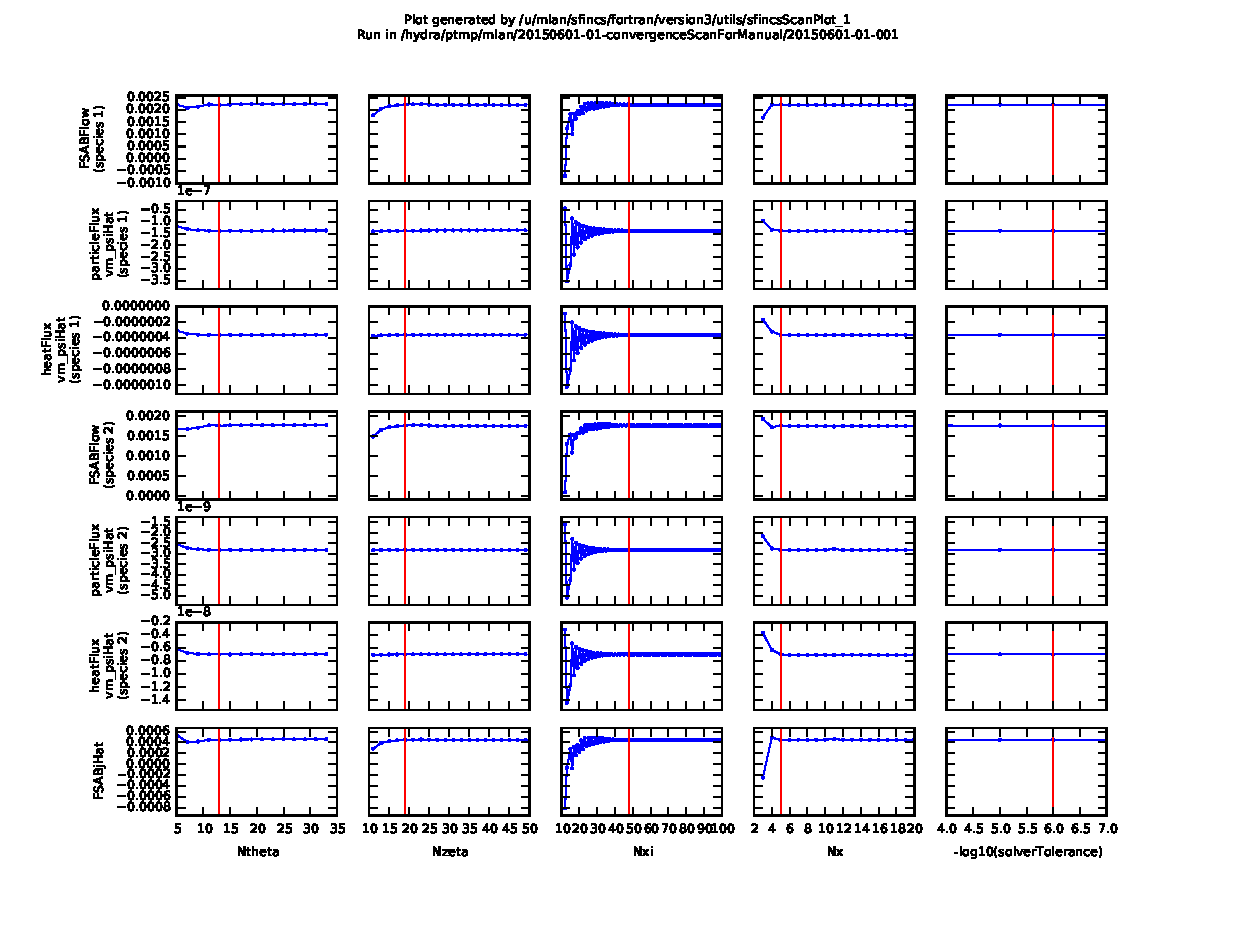
\includegraphics[width=1.0\textwidth]{sfincsConvergenceScan.pdf}
\mycaption{Plot generated by \sfincsScanPlot~showing a resolution convergence scan for the example
{\ttfamily geometryScheme4\_2species\_noEr}.
\label{fig:convergence}}
\end{center}
\end{figure}

To check how well the results of \sfincs~are converged with respect to the resolution
parameters, run \sfincsScan~with \parlink{scanType} = 1.
In this type of scan, a ``base case'' is first run at the
values of \Ntheta, \Nzeta, \Nxi, and \Nx~specified in the input file.
Then, each of these parameters will be varied in turn, holding the other parameters fixed.
The range of \Ntheta~in the scan is specified by the parameters \parlink{NthetaMinFactor},
\parlink{NthetaMaxFactor}, and \parlink{NthetaNumRuns}. 
Each of these three parameters is read by \sfincsScan~rather than by \sfincs~itself,
and so it must be prefaced by {\ttfamily !ss} in the input namelist file.
The ranges of \Nzeta, \Nxi, and \Nx~are set by parameters with analogous names,
as detailed in section \ref{sec:scanType1Parameters}.

For example, suppose you initially run \sfincsScan~with \Ntheta = 15, 
\parlink{NthetaMinFactor} = 0.7, \parlink{NthetaMaxFactor} = 1.5, and 
\parlink{NthetaNumRuns} = 5.
This will generate \sfincs~runs at \Ntheta = 11, 13, 15 (the base case), 19, and 23.
Notice that \sfincsScan~automatically ensures that only odd values are used.
(Only odd values of \Ntheta~and \Nzeta~are used internally in \sfincs.)
The maximum and minimum values for the scan, 11 and 23, are the nearest odd integers
to \Ntheta$\times$\parlink{NthetaMinFactor} and \Ntheta$\times$\parlink{NthetaMaxFactor} respectively.
Notice also that there are `gaps' at  \Ntheta = 17 and 21 since \sfincsScan~attempts to space the values
logarithmically rather than uniformly.

In addition to the 4 resolution parameters above, \sfincsScan~also allows the parameters
\parlink{solverTolerance}, \parlink{xMax}, and \parlink{NxPotentialsPerVth}
to be scanned.  The last two of these parameters are not used for the default \parlink{xGridScheme}
so it is usually unnecessary to scan them.  It is also usually unnecessary to scan \parlink{solverTolerance}
since the default value is usually robust.

A directory will be created for each run.  Each directory will contain
a copy of {\ttfamily input.namelist} in which \Ntheta, \Nzeta, \Nx, or \Nxi~has been
altered appropriately by \sfincsScan. Each directory will also contain a job file for the run.

You do not need to scan all variables. For example, if you do not wish to scan \Nx,
you can either set \parlink{NxNumRuns} = 0, or you can not specify
\parlink{NxNumRuns} in the {\ttfamily input.namelist} file.

Once the individual runs in the scan have begun to finish, you can plot the results by running \sfincsScanPlot.
You can plot the results before all the runs in the scan finish, although at least the base case
run must be completed.  Different quantities will be displayed depending on
\parlink{RHSMode} and \parlink{includePhi1}.

Typical convergence behavior is illustrated in figure \ref{fig:convergence},
showing the results of \sfincsScan~and \sfincsScanPlot~for the example
{\ttfamily geometryScheme4\_2species\_noEr}.
In this figure, a very large number of runs are included in the scan,
more than you would likely include in routine use of the code.
The red vertical lines emphasize the ``base case'' resolution parameters.
In each figure the spread is printed, defined as the maximum value $-$ minimum value,
divided by the value half-way between maximum and minimum.
If some runs have resolution below the base resolution,
the spread is also computed and printed
excluding runs below the base case resolution. (This is the second percentage printed in each plot,
and is usually more important than the first spread percentage.)
For all parameters scanned, the physical output quantities (particle flux, heat flux, etc)
do not visibly change on the scale of the plots when any of the resolution parameters
are increased beyond the base case value.  Indeed, the spread for each output quantity is $\le$ 3.5\%
when any resolution parameter is increased.
Thus, the results in the base case are well converged,
and so we can believe the results.
Observe in the figure that the output quantities tend to oscillate when \Nxi~is incremented by 1 and insufficient
\Nxi~is used. Results for even and odd \Nxi~converge to the same value, as one would hope.

\begin{figure}
\begin{center}
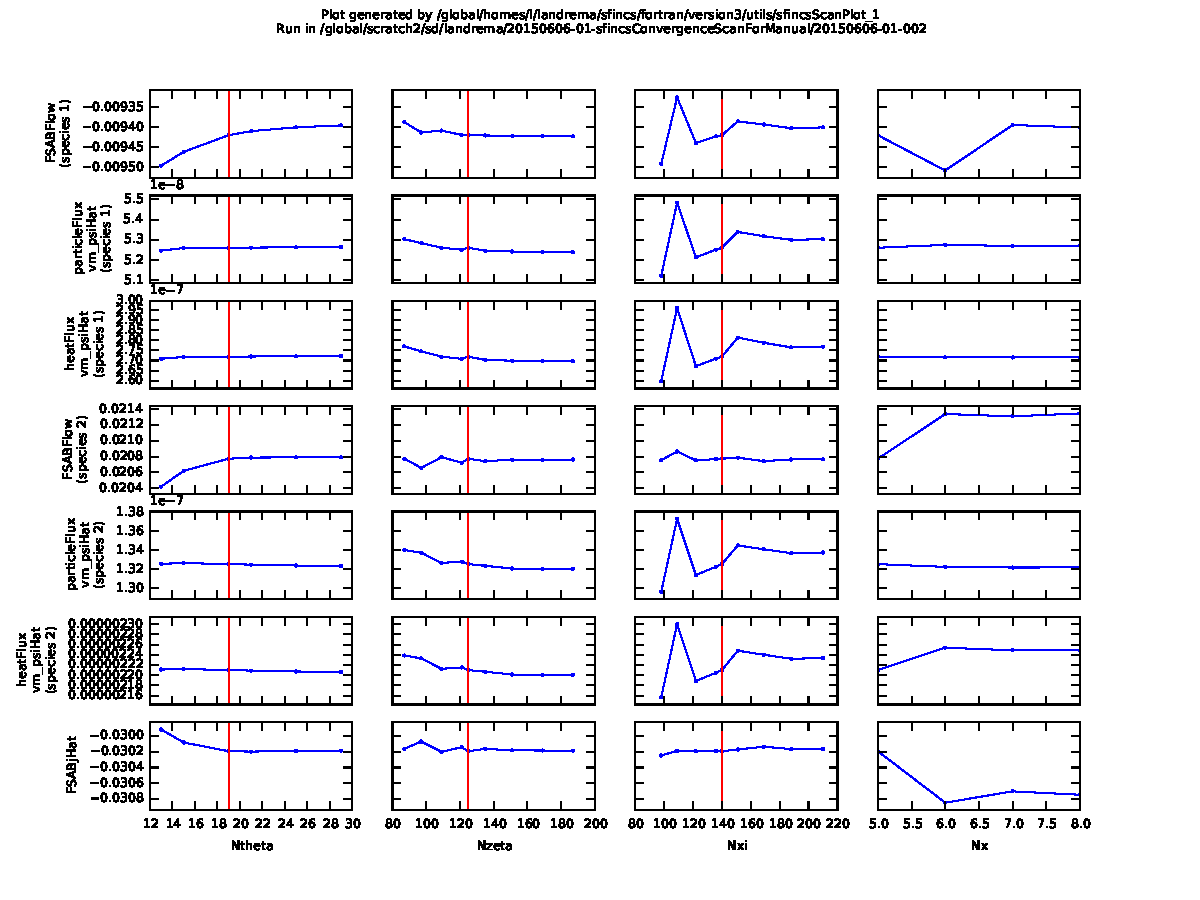
\includegraphics[width=1.0\textwidth]{sfincsConvergenceScan2.pdf}
\mycaption{Plot generated by \sfincsScanPlot~showing a typical resolution convergence scan for W7-X,
as you might generate during routine use of \sfincs.
\label{fig:convergence2}}
\end{center}
\end{figure}

For routine use of the code, it is not necessary to include as many
runs in the convergence scan as shown in figure \ref{fig:convergence},
and so a more typical routine scan would look like figure \ref{fig:convergence2}.
This scan is for a pure hydrogen plasma in the W7-X standard configuration, using \parlink{rN} = 0.19,
$n_e$ = $10^{20}$ m$^{-3}$, $T_i$ = 3.6 keV, and $T_e$ = 5.5 keV.
Notice the vertical scales in figure \ref{fig:convergence2} have suppressed zeros.
For all of the physical output quantities, the spread beyond the base case is $\le$ 3.4\%,
i.e. results change by no more than this percentage when each resolution
parameter is increased by 50\%. Hence we can conclude that 
the results are suitably converged at the base case resolution parameters.
The \sfincs~resolution parameters and \sfincsScan~parameters used for this scan were as follows:\\
{\ttfamily
\Ntheta = 19 \\
!ss \parlink{NthetaMinFactor} = 0.7 \\
!ss \parlink{NthetaMaxFactor} = 1.5 \\
!ss \parlink{NthetaNumRuns} = 6 \\
\Nzeta = 125 \\
!ss \parlink{NzetaMinFactor} = 0.7 \\
!ss \parlink{NzetaMaxFactor} = 1.5 \\
!ss \parlink{NzetaNumRuns} = 8 \\
\Nxi = 140 \\
!ss \parlink{NxiMinFactor} = 0.7 \\
!ss \parlink{NxiMaxFactor} = 1.5 \\
!ss \parlink{NxiNumRuns} = 8 \\
\Nx = 5 \\
!ss \parlink{NxMinFactor} = 1 \\
!ss \parlink{NxMaxFactor} = 1.6 \\
!ss \parlink{NxNumRuns} = 4 \\
}
These \sfincsScan~parameters are good for routine convergence tests, although the \sfincs~parameters proper
(\Ntheta, \Nzeta, \Nxi, and \Nx) should be tailored to your application.

If you wish to add more runs to the scan at a later time,
you can alter the relevant \sfincsScan~parameters in the original {\ttfamily input.namelist}~file
and run \sfincsScan~again from the original directory.  The \sfincsScan~code will automatically detect which runs
have already been submitted, so duplicate runs will not be generated.
For example, consider the scan of \Ntheta~described at the start of this section,
and suppose you wish to fill in the gaps at \Ntheta = 17 and 21 in the original scan.
To do this, you could set \parlink{NthetaNumRuns} to a large number like 100
and re-run \sfincsScan.  Since \sfincsScan~intelligently avoids duplication,
the only new runs generated will be  \Ntheta = 17 and 21.

If you are ultimately intending to scan $E_r$, you probably only need to run a convergence scan
at a single value of $E_r$.  This is because the resolution requirements of \sfincs~are not sensitive to
$E_r$, as discussed above.
Also, if you are ultimately intending to run \sfincs~at a range of minor radii,
it is reasonably to only run a convergence scan at a single radius close to the magnetic axis.
This is because the typically peaked shape of the temperature profile means that
collisionality is lowest near the axis.  Since the resolution requirements of \sfincs~are most
demanding at low collisionality, then if the code is converged at the radius of lowest collisionality,
it should be converged at all radii.

\section{Examples of resolution requirements}

To estimate the appropriate resolution parameters for various circumstances, you can look at
the examples in the \path{sfincs/fortran/version3/examples/} directory. 
Some other examples of appropriate resolution parameters are given in the following sections.

\subsection{W7-X with anticipated experimental density and temperature}
\label{sec:w7xresolution}

The following parameters have been extensively tested with W7-X geometry for densities near $10^{20}$ m$^{-3}$
and temperatures up to 6 keV, and found to give convergence to $\sim 3$\% (as shown in figure \ref{fig:convergence2}):\\
{\ttfamily
\Ntheta = 19 \\
\Nzeta = 125 \\
\Nxi = 140 \\
\Nx = 5 \\
}
Note that at lower temperature and/or higher density, the collisionality will be higher,
so comparable convergence could be achieved at lower \parlink{Nzeta} and \parlink{Nxi}.
Conversely, at higher temperatures and/or lower desntiy, the collisionality will be lower,
so comparable convergence would likely require higher  \parlink{Nzeta} and \parlink{Nxi}.

\subsection{Figure 3 of the original SFINCS paper}

For figure 3 in Ref \cite{sfincsPaper}, corresponding to a pure plasma in W7-X with $n = 6.6\times 10^{19}$ m$^3$ and $T_i = T_e = 1$ keV,
the calculations used\\
{\ttfamily
\Ntheta = 19 \\
\Nzeta = 59 \\
\Nxi = 60 \\
\Nx = 5. \\
}
Note the lower values of  \parlink{Nzeta} and \parlink{Nxi} used compared to section \ref{sec:w7xresolution},
which were sufficient since the temperatures were lower.

\subsection{Figure 4 of the original SFINCS paper}

For figure 4 in Ref \cite{sfincsPaper}, corresponding to a collisionality scan in LHD,
the following resolution parameters were used:

\centerline{
\begin{tabular}{c|c|c|c|c}
\parlink{nuPrime} & \Ntheta & \Nzeta & \Nxi & \Nx \\
\hline
0.001 & 85 & 41 & 103 & 5 \\
0.01 & 21 & 25 & 70 & 5 \\
0.1 & 15 & 13 & 37 & 5 \\
0.3 & 15 & 13 & 34 & 6 \\
1 & 13 & 13 & 13 & 8 \\
10 & 15 & 13 & 13 & 8 \\
100 & 15 & 13 & 13 & 8
\end{tabular}
}

\subsection{Figure 5 of the original SFINCS paper}

For figure 5 in Ref \cite{sfincsPaper}, corresponding to a collisionality scan in W7-X,
the following resolution parameters were used:

\centerline{
\begin{tabular}{c|c|c|c|c}
\parlink{nuPrime} & \Ntheta & \Nzeta & \Nxi & \Nx \\
\hline
0.001 & 29 & 83 & 180 & 5 \\
0.01  & 11 & 64 & 100 & 5 \\
0.1   & 11 & 37 & 37  & 5 \\
0.3   & 11 & 29 & 30  & 5 \\
1     & 13 & 31 & 24  & 6 \\
10    & 13 & 35 & 12  & 7 \\
100   & 11 & 37 & 13  & 8
\end{tabular}
}
